% Requires \usepackage{graphicx} in the manuscript preamble.
\begin{figure*}[t]
    \centering
    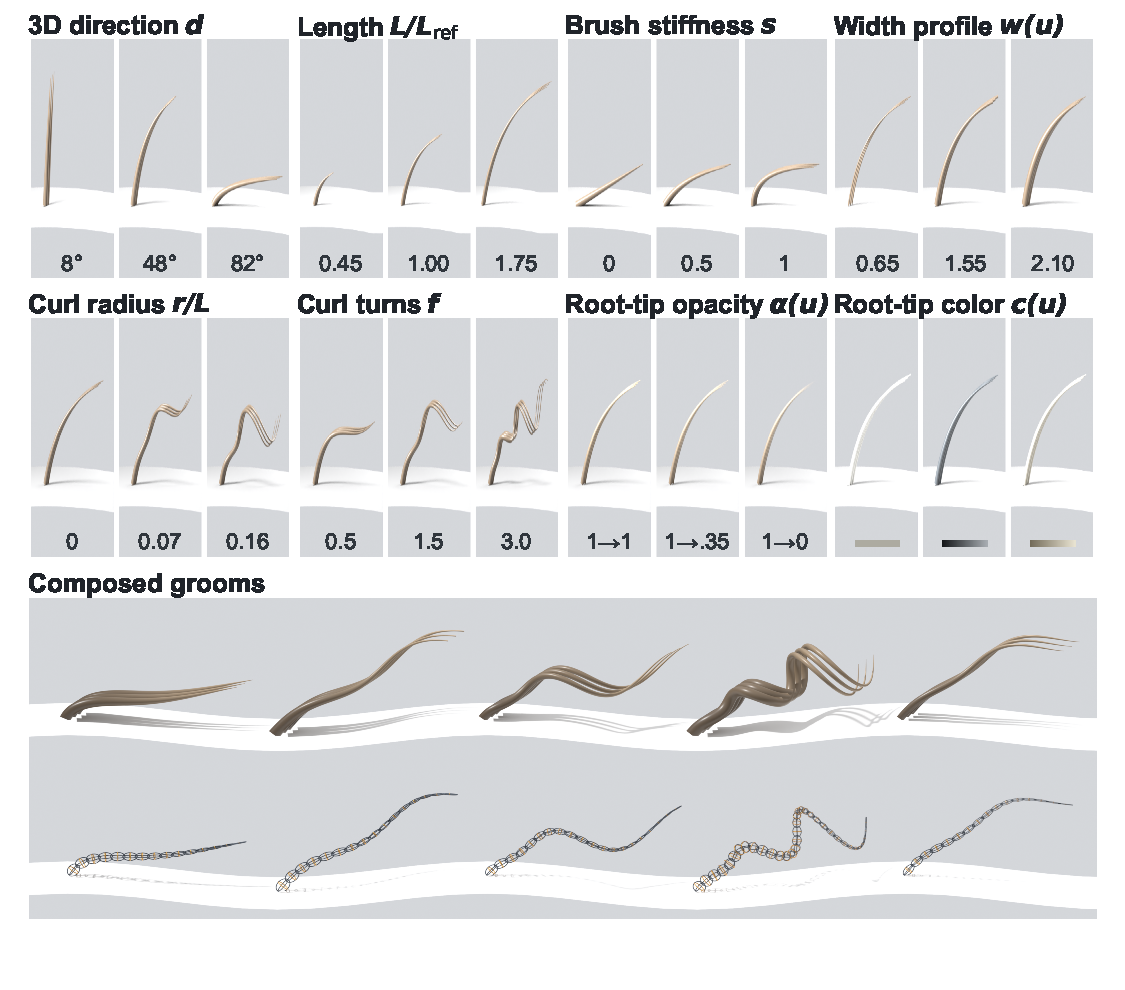
\includegraphics[width=\textwidth]
    {method/fig_parametric_groom_controls.pdf}
    \caption{\textbf{Interpretable differentiable groom controls.}
    Single-variable sweeps show the effects of 3D direction, length, brush
    stiffness, width profile, curl radius, curl turns, root-to-tip opacity,
    and root-to-tip color. The displayed geometric sweeps use
    $\hat{L}=L/L_{\mathrm{ref}}$ and $\hat{r}=r/L$. Each strand is rendered over a shallow convex
    receiver to expose its three-dimensional shape and contact shadow. The
    composed examples combine multiple controls; the aligned lower row shows
    the corresponding adaptive anisotropic Gaussian initialization after all
    geometric deformation.}
    \label{fig:parametric-groom-controls}
\end{figure*}
